 \documentclass[11pt, oneside]{article} 
\usepackage{geometry}
\geometry{letterpaper} 
\usepackage{graphicx}
	
\usepackage{amssymb}
\usepackage{amsmath}
\usepackage{parskip}
\usepackage{color}
\usepackage{hyperref}

\graphicspath{{/Users/telliott_admin/Dropbox/Tex/png/}}
% \begin{center} 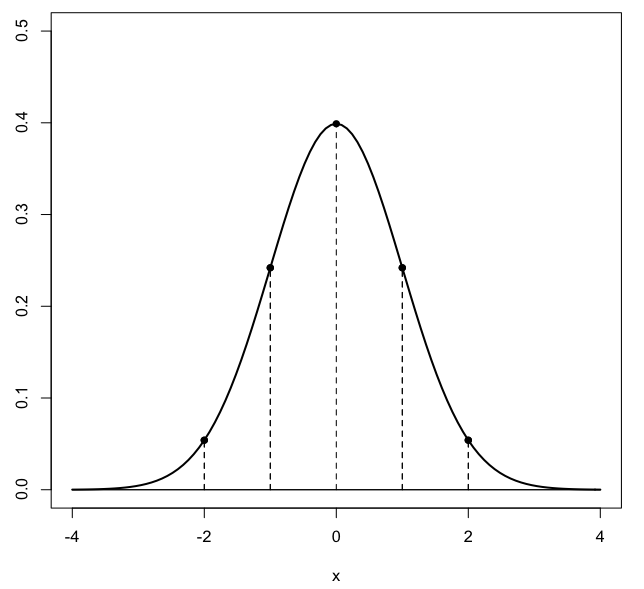
\includegraphics [scale=0.4] {gauss3.png} \end{center}

\title{Sequences}
\date{}

\begin{document}
\maketitle
\Large

A sequence in $\mathbb{R}$ is a list or ordered set $(a_1, a_2, a_3, \dots)$ of real numbers.

A sequence of numbers $(a_n)$ starts at a specific place, with a particular first term $a_1$ and then goes on forever.  Usually, there will be some kind of pattern:
\[ (a_n) = a_1,  a_2, a_3, \dots a_n, \dots \]
\[ 1,2,3 \dots \]
or whatever.  

Note the difference between notation for the nth term---$a_n$, and the sequence itself $(a_n)$.

Technically a sequence is a function from the natural numbers to the reals ($f : \mathbb{N} \rightarrow \mathbb{R}$).

A sequence may be defined by a specific formula like $1/n$ or it may be described by a recurrence relation like $a_{n+2} = a_n + a_{n+1}$ (the Fibonacci numbers) or
\[ a_{n+1} = a_n + \frac{1}{n^2} = \frac{\pi^2}{6} \]
In the case of a recurrence we must specify the first (or first and second in the case of Fibonacci) terms.

\subsection*{monotonic sequences}
$\bullet$  The sequence ($a_n$) is \emph{increasing} $\iff \forall \ n \in N, \ \ \ a_{n+1} \ge a_n$

Note the $\ge$.  A monotonic sequence that increases need not be \emph{strictly increasing}.  

$\bullet$  A sequence is \emph{monotonic} $\iff$ it is increasing or decreasing.

So there are two different types of monotonic sequences, those that go up and those that go down.  For the most part, monotonic sequences that are increasing are mirror images of the ones that decrease, so we can concentrate on the first class.

\subsection*{bounded sequences}

If we can find a number $M$ which is never exceeded by any term in the sequence, then it is bounded above.  

$\bullet$  The sequence ($a_n$) is \emph{bounded above} $\iff$
\[ \exists \ M \in \mathbb{R} \ | \ \forall \ n \in \mathbb{N}, a_n \le M \]

$\bullet$  Any sequence that has an upper bound has many upper bounds (e.g. $M+1$ is also an upper bound).

$\bullet$  The sequence ($a_n$) is \emph{bounded} $\iff \exists \ M > 0 \ | \ \forall \ n \in \mathbb{N}, |a_n| \le M$  

A sequence is bounded if it is bounded above \emph{and} bounded below.
\begin{center} 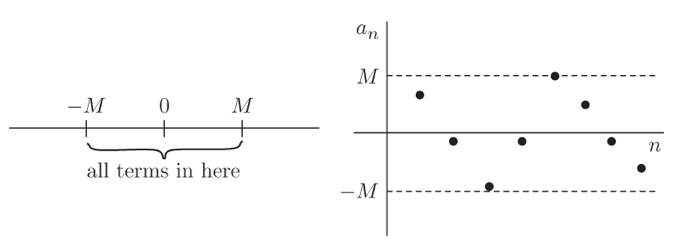
\includegraphics [scale=0.5] {bounded1.png} \end{center}

\subsection*{convergent sequences}
$\bullet$  The sequence ($a_n$) \emph{converges} to $a$  $\iff$
\[ \forall \ \epsilon > 0, \ \exists \ N \in \mathbb{N} \ | \ \forall \ n > N, |a_n - a| < \epsilon \]
\begin{center} 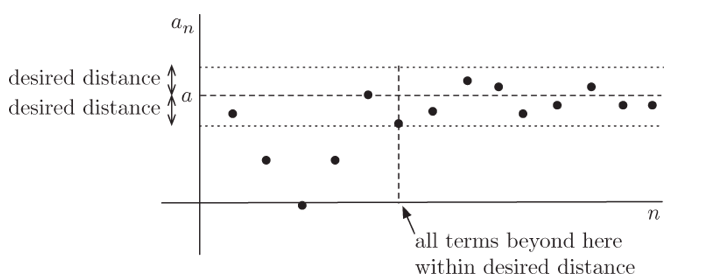
\includegraphics [scale=0.5] {convergent1.png} \end{center}

The early behavior of a sequence is irrelevant.  The requirement is that at some point (for index $n > N$), all the terms after $a_n$ must be closer than $\epsilon$ to the value $a$:  that is $|a_n - a| < \epsilon$.  The terms may be either $> a$ or $< a$.

$\epsilon$ can be chosen as small as we like, and the sequence must get as close as $\epsilon$ to the value $a$.

$\bullet$  Suppose that $(a_n)$ is a sequence and $L$ is a real number. If for all $\epsilon > 0$, we can find a term in the sequence such that it differs from $L$ by less than $\epsilon$ 
\[ |a_n - L | < \epsilon \]
and the same is true for all subsequent terms, then the sequence $(a_n)$ is \emph{convergent} and $L$ is its \emph{limit}.

\subsection*{convergent sequences}

$\bullet$ Any convergent sequence has a \emph{least upper bound} and a greatest lower bound.

\textbf{Proof}:

Suppose that the sequence $(a_n) \rightarrow \alpha$.  Take $\epsilon = 1$.  Simply choose $N$ so that when $n > N$, we have $a_n$ within $1$ of $\alpha$.  ($|a_n - \alpha| < \epsilon = 1$).

Apart from the terms $(a_1, \dots a_N)$ we have that all the terms of the sequence are bounded by $\alpha + 1$ and $\alpha - 1$.  So an upper bound for the sequence is $max(a_1, \dots a_N, \alpha + 1)$.

\subsection*{examples}

$\circ$  $(1, 1/2, 1/3, \dots)$ converges to $0$.

\textbf{Proof}:  Given $\epsilon$ the Archimedean property guarantees we can find $1/N \le \epsilon$.  Then if $n > N$ we have
\[ \frac{1}{n} < \frac{1}{N} \le \epsilon \]

$\circ$  The sequence $(1, 2, 3, \dots)$ is not bounded.  Any unbounded sequence fails to converge.

$\circ$  The sequence
\[ 1, 1 + \frac{1}{2}, 1 + \frac{1}{2} + \frac{1}{3}, 1 + \frac{1}{2} + \frac{1}{3} +  \frac{1}{4}, \dots \]
is the sequence of partial sums of the harmonic series, which does not converge.

\subsection*{bounded, monotone sequences}

We combine the previous concepts of a bounded monotone sequence and convergence:

\textbf{Axiom}  (Monotone Sequence Property). \emph{Any bounded monotone sequence converges.}

Beck:
\begin{quote}This axiom (or one of its many equivalent statements) gives arguably the most important property of the real number system; namely, that we can, in many cases, determine that a given sequence converges without knowing the value of the limit. In this sense we can use the sequence to define a real number.\end{quote}

$\bullet$  A bounded monotonic increasing sequence converges, and it converges to its least upper bound.

Let $\alpha$ be the least upper bound of the sequence.

Given $\epsilon > 0$, we will show that all the terms of the sequence after some finite number of initial terms are in the interval $(\alpha - \epsilon, \alpha + \epsilon)$.

$\circ$  Since $\alpha + \epsilon$ is an upper bound of the sequence, all the terms certainly satisfy $a_n < \alpha + \epsilon$.

$\circ$  And since $\alpha - \epsilon$ is \emph{not} an upper bound of the sequence, we must have $a_N > \alpha - \epsilon$ for some $N$.

$\circ$  But then all the later terms $a_n$ (for $n > N$)  will satisfy $a_n > \alpha - \epsilon$ (by the montonic property), and so we have our condition for convergence.

\end{document}